\section{phase$\_$5}

	\begin{itemize}

	\item
	
	第五关的汇编代码如下:
		
	\lstinputlisting[language={[x86masm]Assembler}]{sources/phase_5.asm}
	
	\item
		
	\lstinputlisting[language={[x86masm]Assembler}]{sources/phase_5_part_1.asm}
	
	首先,我们发现它调用了\textbf{string$\_$length}这个函数,并且将返回值与$6$进行比较,不相等的话炸弹会爆炸。查看\textbf{string$\_$length}的代码发现,它的功能为返回一个字符串的长度。
	
	因此,我们得到了第一个限制条件:需要输入一个长度为6的字符串。

	\item
		
	\lstinputlisting[language={[x86masm]Assembler}]{sources/phase_5_part_2.asm}
	
	这里是一个循环,循环变量是$\%eax$,范围从0到5。

	\item
	
	\lstinputlisting[language={[x86masm]Assembler}]{sources/phase_5_part_3.asm}
	
	\textbf{movsbl}这个语句的意思为,将位于$Mem[\%ebx + \%eax]$处地址的数据最低位取出,进行符号位扩展后送入$\%edx$中,结合后面一句\textbf{and  $\$0xf, \%edx$},以及$\%$ebx即为输入字符串的首地址,可以发现这句话的意思是取出输入字符串第\textbf{$\%$eax}位ASCII码的后四位。	
	
	\item
	\lstinputlisting[language={[x86masm]Assembler}]{sources/phase_5_part_4.asm}
	
		
	这个语句将刚刚取出的值作为下标,在从\textbf{0x8049a7c}开始的数组中进行寻值,并将结果构成新的字符串压入栈中。于是,我们调用gdb命令,查看\textbf{0x8049a7c}地址对应的值。
	
	\begin{figure}[h]
		\centering
			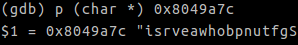
\includegraphics[scale=0.8]{images/phase_5_part_5.png}
	\end{figure}	
	
	这里相当于是一个密码加密的过程,即将每一个原先的字母用一个一一对应的字母替换。

	\item
		
	\lstinputlisting[language={[x86masm]Assembler}]{sources/phase_5_part_6.asm}
	
	这里又向栈中压入了一个\textbf{0x8049a52}地址中的数据,并且调用\textbf{strings$\_$not$\_$equal}函数。根据之前的分析,如果传入的两个字符串不等,炸弹就会爆炸。因此,我们生成的字符串应该与\textbf{0x8049a52}地址中的相同。
	
	\item
	
	于是调用gdb,查看\textbf{0x8049a52}地址中的内容:
	\begin{figure}[h]
		\centering
			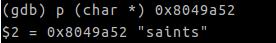
\includegraphics[scale=0.8]{images/phase_5_part_7.png}
	\end{figure}	
		
	\item
		
	因此,我们只需要生成“saints”这个字符串即可。根据索引表,“saints”这六个字母对应的索引值分别为1, 5, 0, 11, 13, 1。
	
	我们只需要输入六个ASCII码低4位为这六个值的字符即可。于是选用 \textbf{a, e, 0, k, m, a}。
	
	\end{itemize}
	
	输入\textbf{ae0kma},顺利过关。
	
	\begin{figure}[h]
		\centering
			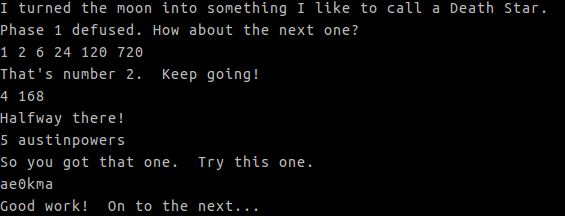
\includegraphics[scale=0.8]{images/phase_5_success.png}
	\end{figure}	